% --------------------------------------------------------------
% This is all preamble stuff that you don't have to worry about.
% Head down to where it says "Start here"
% --------------------------------------------------------------
 
\documentclass[12pt]{article}
 
\usepackage[margin=1in]{geometry} 
\usepackage{amsmath,amsthm,amssymb}
\usepackage[margin=1in]{geometry} 
\usepackage{amsmath,amsthm,amssymb}
\usepackage[T1]{fontenc} %escribe lo del teclado
\usepackage[utf8]{inputenc} %Reconoce algunos símbolos
\usepackage{lmodern} %optimiza algunas fuentes
\usepackage{graphicx}
\graphicspath{ {images/} }
\usepackage{tikz}
\usepackage[]{algorithm2e}
\usepackage{hyperref} % Uso de links
 
\newcommand{\N}{\mathbb{N}}
\newcommand{\Z}{\mathbb{Z}}
 
\newenvironment{theorem}[2][Theorem]{\begin{trivlist}
\item[\hskip \labelsep {\bfseries #1}\hskip \labelsep {\bfseries #2.}]}{\end{trivlist}}
\newenvironment{lemma}[2][Lemma]{\begin{trivlist}
\item[\hskip \labelsep {\bfseries #1}\hskip \labelsep {\bfseries #2.}]}{\end{trivlist}}
\newenvironment{exercise}[2][Exercise]{\begin{trivlist}
\item[\hskip \labelsep {\bfseries #1}\hskip \labelsep {\bfseries #2.}]}{\end{trivlist}}
\newenvironment{problem}[2][Problem]{\begin{trivlist}
\item[\hskip \labelsep {\bfseries #1}\hskip \labelsep {\bfseries #2.}]}{\end{trivlist}}
\newenvironment{question}[2][Question]{\begin{trivlist}
\item[\hskip \labelsep {\bfseries #1}\hskip \labelsep {\bfseries #2.}]}{\end{trivlist}}
\newenvironment{corollary}[2][Corollary]{\begin{trivlist}
\item[\hskip \labelsep {\bfseries #1}\hskip \labelsep {\bfseries #2.}]}{\end{trivlist}}

\newenvironment{solution}{\begin{proof}[Solution]}{\end{proof}}
 
\begin{document}
 
% --------------------------------------------------------------
%                         Start here
% --------------------------------------------------------------
 
\title{Learning Coursework: Task 1 report}


\maketitle
\newpage
\subsection*{1.2 - Correlation matrix interpretation}

\begin{figure}[!htb]
\centering
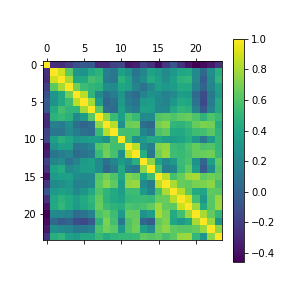
\includegraphics[scale=0.8]{task1_2_covm.png}
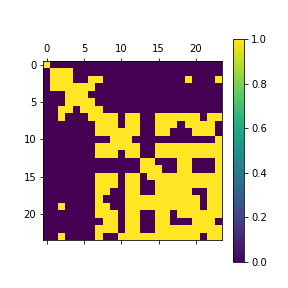
\includegraphics[scale=0.8]{task1_2_covm_stepped.png}
\caption{Covariance matrix heatmaps - the full one and one with an applied step function ($1$ if $> 0.5$, $-1$ if $< 0.5$, $0$ otherwise)}
\label{task1_2_covm}
\end{figure}

\subsubsection*{Negative correlations}
As we can see on Figure \ref{task1_2_covm}, the only feature that is negatively correlated with others is the feature with index $0$ (dark blue bars on the upper and left edges of the matrix). These are weak negative correlations, as they are bounded below by about $-0.4$.
\subsubsection*{Positive correlations}
As we can see in the second plot on Figure \ref{task1_2_covm}, there are many features with high positive correlations ($>0.5$, seen in yellow). We can observe two clusters of features that are mostly correlated with each other - features in $[1,6]$ and features in $[7,23]$ (the rectangles that contain all the pairs of features within these intervals are mostly yellow).

\newpage
\subsection*{1.3}

\begin{figure}[!htb]
\centering
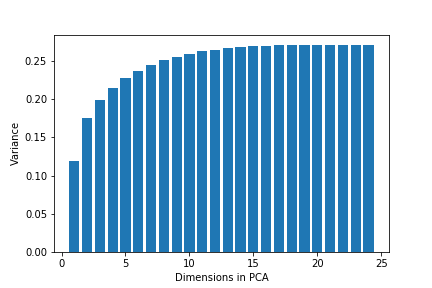
\includegraphics[scale=0.8]{task1_3b_cumvar_graph.png}
\caption{\textbf{Task 1.3b - Cumulative variance graph}}
\end{figure}

\begin{figure}[!htb]
\centering
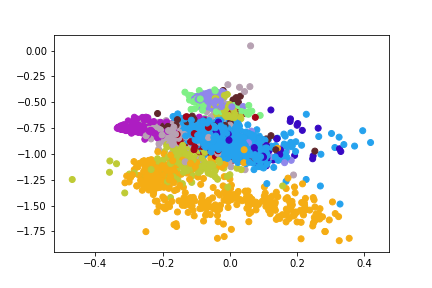
\includegraphics[scale=1]{task1_3c_scatter_classes.png}
\caption{\textbf{Task 1.3c - 2D-PCA plane}}
\end{figure}

\newpage

\subsection*{1.4b - Accuracy vs Covariance Matrix Type}
\begin{tabular}{|c|c|c|c|}
\hline 
\textbf{CovKind} & \emph{Full} & \emph{Diagonal} & \emph{Shared} \\ 
\hline 
\textbf{Accuracy} & 90.101\% & 83.028\% & 88.270\% \\ 
\hline 
\end{tabular} 

\subsection*{1.5 - Regularisation parameter analysis}

\begin{figure}
\centering
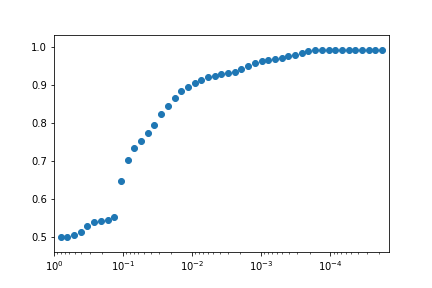
\includegraphics[scale=1]{task1_4c_epsilons_accuracy.png}
\caption{\textbf{1.5 - Impact of the epsilon on accuracy}; logarithmically scaled x-axis}}
\label{epsilon_analysis}
\end{figure}

Intuitively, we would expect the accuracy to drop when taking bigger epsilons, as this makes the approximation of the covariance matrix worse. Figure \ref{epsilon_analysis} confirms that; accuracy increases when we take smaller epsilons. What is more, the plot becomes nearly flat for $x<10^{-4}$, so there is no benefit from taking smaller epsilons than that.

\end{document}

